\documentclass[../qm.tex]{subfiles}
\begin{document}
		\section{The Classical Definition}
		A microcanonical ensemble is an ensemble which is \textit{isolated} from the universe.\\
		Such system can be described by a fixed number of particles in a fixed volume $V$ with energies lying in an interval $[E,E+\delta]$, with an Hamiltonian $\ham(q,p)$. What we wish to find is the classical density matrix of this system (i.e. the distribution function for such system).\\
		We already know that the region of phase space (the space composed by all the coordinates and the conjugated momenta) occupied by such system must be an hypervolume limited by two hypersurfaces with the following equations
		\begin{equation}
			\begin{aligned}
				\ham(q,p)&=E\\
				\ham(q,p)&=E+\delta
			\end{aligned}
			\label{eq:hypervolumeinphasespace}
		\end{equation}
		This hypervolume is called \textit{energy shell}. Since this state must tend to an equilibrium, we know already that every single microstate must be equiprobable and if they weren't, the density matrix would depend from other factors and would end up not commuting with the Hamiltonian, and bringing the system to never actually reach equilibrium.\\
		Such ensemble is called the \textit{microcanonical ensemble}, and the associated \textit{microcanonical distribution function} has the following form
		\begin{equation}
			\rho_{MC}(q,p)=\begin{dcases}
						\frac{1}{\Omega(E)\delta}&E\le\ham(q,p)\le E+\delta\\
						0&\ham(q,p)\notin[E,E+\delta]
					\end{dcases}
			\label{eq:microcanonicaldensity}
		\end{equation}
		Where $\Omega(E)\delta$ is the volume occupied in the phase space, which we will now identify as $\Gamma^{2n}$. In the limit $\delta\to0$ we have
		\begin{equation}
			\rho_{MC}(q,p)=\frac{1}{\Omega(E)}\delta\left( E-\ham(q,p) \right)
			\label{eq:rhomclimitdelta}
		\end{equation}
		From this, we can immediately determine $\Omega(E)$ by calculating the normalization of $\rho_{MC}(q,p)$.
		\begin{equation}
			\int_{}^{}\rho_{MC}(q,p)\diff{\mu}=\frac{1}{h^{3N}N!}\int_{}^{}\rho_{MC}(q,p)\ddiff{q}{p}=1
			\label{eq:rhonormalization}
		\end{equation}
		Where we used the Lebesgue measure $\diff{\mu}=(h^{3N}N!)^{-1}\ddiff{q}{p}$, where $h$ is a constant that comes out from the need of having a discrete phase space (see thermodynamics) and the factor $N!$ is a factor discovered by Gibbs, which results from the indistinguishability of the particles. Its absence would let the existence of an entropy of mixing gases, this is referred in literature as \textit{Gibbs' paradox}.\\
		From what we have then defined before, we now can write that the function $\Omega(E)$ can be evaluated with the following integral
		\begin{equation}
			\Omega(E)=\int_{}^{}\delta\left( E-\ham(q,p) \right)\diff{\mu}
			\label{eq:omegaedirectcalculus}
		\end{equation}
		This function is also referred as the \textit{phase surface} of the system.\\
		We can also define the volume of the region $\cc{\Omega}(E)$ as follows
		\begin{equation}
			\cc{\Omega}(E)=\int_{}^{}\Theta\left( E-\ham(q,p) \right)\diff{\mu}
			\label{eq:phasevolume}
		\end{equation}
		From functional analysis, we already know that the following relation then holds
		\begin{equation}
			\Omega(E)=\derivative{\cc{\Omega}}{E}
			\label{eq:omegaomegabarrel}
		\end{equation}
		Comparing both $\cc{\Omega}(E)$ and $\Omega(E)\delta$ we can see that
		\begin{equation*}
			\log\left( \Omega(E)\delta \right)=\log\left( \Omega(E) \right)+\order{\log\left( \frac{E}{n\delta} \right)}
		\end{equation*}
		Therefore, for large values of $n$ we can write
		\begin{equation}
			\Omega(E)\delta=\cc{\Omega}(E)
			\label{eq:ccomegaomegauguagliance}
		\end{equation}
		\section{The Quantum Definition}
		Quantum mechanically, the definition of a microcanonical ensemble is an isolated system with an Hamiltonian $\opr{\ham}$ and associated energy eigenvalues $E_n$ with eigenstate $\ket{n}$. The microcanonical density operator then is defined as follows
		\begin{equation}
			\opr{\rho}_{MC}=\sum_np\left( E_n \right)\ket{n}\bra{n}
			\label{eq:mcdopr}
		\end{equation}
		Where the probability of each energy level $E_n$ analogously to classical mechanics, is defined as follows
		\begin{equation}
			p(E_n)=\begin{dcases}
				\frac{1}{\Omega(E)\delta}&E\le E_n\le E+\delta\\
				0&E_n\notin[E,E+\delta]
			\end{dcases}
			\label{eq:probabilitystatedoprmc}
		\end{equation}
		From the normalization of $\dopr_{MC}$ we get
		\begin{equation}
			\begin{aligned}
				\dopr&=\frac{1}{\Omega(E)}\opr{\delta}\left( \opr{\ham}-E \right)\\
				\Omega(E)&=\trace{\opr{\delta}}\left( \opr{\ham}-E \right)
			\end{aligned}
			\label{eq:OmegaEquantummc}
		\end{equation}
		Or introducing a new notation
		\begin{equation}
			\Omega(E)=\frac{1}{\delta}\qsum_{\{\ket{n}\}}1
			\label{eq:sumone}
		\end{equation}
		Where the $\sum'$ symbol indicates that the sum is restricted only to the energy eigenvalues contained in the energy shell
		\section{Entropy, Temperature and Pressure}
		Let $\rho$ be an arbitrary density matrix for a system. The \textit{entropy} of this system is defined as follows
		\begin{equation}
			S=-k_B\trace\left( \rho\log(\rho) \right)=-k_B\expval{\log(\rho)}
			\label{eq:generalentropy}
		\end{equation}
		From this definition, all properties of classical entropy, already well known from macroscopic thermodynamics follow.\\
		This definition is easily transferable to the quantum definition (where the entropy is usually called the \textit{Von Neumann entropy}), through the quantization $\rho(q,p)\to\opr{\rho}$. Another property of entropy can be given immediately. Let $\opr{\rho}$ and $\opr{\rho}_1$ be two density operators, then
		\begin{equation}
			\trace\left( \opr{\rho}\left( \log(\opr{\rho}_1)-\log(\opr{\rho}) \right) \right)\le0
			\label{eq:entropypropertynegativetrace}
		\end{equation}
		Diagonalizing both operators, we can write
		\begin{equation*}
			\begin{aligned}
				\trace\left( \opr{\rho}\left( \log(\opr{\rho}_1)-\log(\opr{\rho}) \right) \right)&=\sum_nP_n\bra{n}(\log(\opr{\rho}_1))-\log(P_n)\ket{n}=\sum_nP_n\bra{n}\log\left( \frac{\opr{\rho}_1}{P_n} \right)\ket{n}=\\
				&=\sum_n\sum_\nu P_n\bra{n}\ket{\nu}\bra{\nu}\log\left( \frac{P_{1\nu}}{P_n} \right)\ket{\nu}\bra{\nu}\ket{n}\le\\
				&\le\sum_n\sum_\nu P_n\bra{n}\ket{\nu}\bra{\nu}\left( \frac{P_{1\nu}}{P_n}-1 \right)\ket{\nu}\bra{\nu}\ket{n}=\\
				&=\sum_nP_n\bra{n}\left( \frac{\opr{\rho}_1}{P_n}-1 \right)\ket{n}=\trace(\opr{\rho}_1)-\trace(\opr{\rho})\le0
			\end{aligned}
		\end{equation*}
		\subsection{Entropy of a Microcanonical Ensemble}
		Using the definition of the Von Neumann entropy, we define
		\begin{equation*}
			S_{MC}=-k_B\trace\left( \opr{\rho}_{MC}\log(\opr{\rho}_{MC}) \right)=-k_B\trace\left( \opr{\rho}_{MC}\log\left( \frac{1}{\Omega(E)\delta} \right) \right)
		\end{equation*}
		From the normalization condition of $\opr{\rho}_{MC}$, we obtain
		\begin{equation}
			S_{MC}=k_B\log\left( \Omega(E)\delta \right)
			\label{eq:microcanonicalentropy}
		\end{equation}
		I.e. entropy is proportional to the accessible volume on the phase space (classically) or it's the logarithm of the number of accessible states (quantum mechanical)\\
		\subsection{Temperature and Pressure}
		Let's now define an isolated system composed of two interacting subsystems. The density operator for such system will be
		\begin{equation}
			\opr{\rho}_{MC}=\Omega_{1,2}^{-1}(E)\opr{\delta}\left( \opr{\ham}_1+\opr{\ham}_2-E \right)
			\label{eq:microcanonicalrho}
		\end{equation}
		Indicating the probability that the first system lies at some energy $E_1$ with $\omega(E_1)$, we have
		\begin{equation}
			\omega(E_1)=\expval{\opr{\delta}\left( \opr{\ham}_1-E_1 \right)}=\frac{\Omega_2(E-E_1)\Omega_1(E_1)}{\Omega_{1,2}(E)}
			\label{eq:omegaE1}
		\end{equation}
		Finding the extremal of such function, and putting it back to the definition of the microcanonical entropy, we get
		\begin{equation}
			\pdv{S_2}{E_2}=\pdv{S_1}{E_1}
			\label{eq:closedformentropy}
		\end{equation}
		If we now define the temperature as follows we have
		\begin{equation}
			\frac{1}{T}=\pdv{S}{E}
			\label{eq:temperaturedef}
		\end{equation}
		We have
		\begin{equation*}
			T_1=T_2
		\end{equation*}
		Which is the most probable configuration.\\
		Instead for defining pressure, we let the Hamiltonian depend from an external parameter $a$.\\
		We start by writing the volume in the phase space
		\begin{equation}
			\cc{\Omega}(E,a)=\int\Theta\left( E-\ham(a) \right)\diff{\Gamma}
			\label{eq:omegabarpressure}
		\end{equation}
		Taking the total differential, we have
		\begin{equation}
			\diff{\cc{\Omega}}(E,a)=\int_{}^{}\delta\left( E-\ham(a) \right)\left( \diff{E}-\pdv{\ham}{a}\diff{a} \right)=\Omega(E,a)\left( \diff{E}-\expval{\pdv{\ham}{a}}\diff{a} \right)
			\label{eq:diffccOmegaEpressure}
		\end{equation}
		In an alternative way we could write
		\begin{equation*}
			\diff{\log\cc{\Omega}}=\frac{\Omega}{\cc{\Omega}}\left( \diff{E}-\expval{\pdv{H}{a}}\diff{a} \right)
		\end{equation*}
		Inserting the entropy into the equation $S(E,a)=k_B\log(\cc{\Omega}(E,a))$ we have
		\begin{subequations}
			\begin{equation}
				\diff{S}=\frac{1}{T}\left( \diff{E}-\expval{\pdv{\ham}{a}}\diff{a} \right)
				\label{eq:entropydifferentialpressure}
			\end{equation}
			And, thus
			\begin{equation}
				\left\{\begin{aligned}
						\pdv{S}{E}&=\frac{1}{T}\\
						\pdv{S}{a}&=-\frac{1}{T}\expval{\pdv{\ham}{a}}
				\end{aligned}\right.
				\label{eq:entropypressure}
			\end{equation}
			\label{subeq:pressure}
		\end{subequations}
		By taking $a=V$ we then can define pressure.\\
		Let's imagine an ideal gas inside an adiabatic piston with volume $V=LA$, where $L$ is the length of the piston and $A$ it's surface area.\\
		The potential given by this system will be the sum of the single potentials of every $N$ particles
		\begin{equation*}
			V_{wall}=\sum_{i=1}^Nv(x_i-L)
		\end{equation*}
		Where $v$ is a function that is $0$ for $x_i<L$ and infinite for $x_i>L$. By taking the gradient of this potential we then obtain the force applied by each particle on the walls
		\begin{equation}
			F=\sum_iF_i=-\sum_i\pdv{v}{x_i}=\pdv{L}\sum_iv(x_i-L)=\pdv{\ham}{L}
			\label{eq:forceapplied}
		\end{equation}
		Multiplying by $A^{-1}$, we obtain
		\begin{equation}
			P=-\frac{\expval{F}}{A}=\pdv{\ham}{V}
			\label{eq:pressure}
		\end{equation}
		And, therefore, we have
		\begin{subequations}
			\begin{equation}
				\diff{S}=\frac{1}{T}\left( \diff{E}+P\diff{V} \right)
				\label{eq:differentialspiston}
			\end{equation}
			And
			\begin{equation}
				\left\{\begin{aligned}
						\pdv{S}{E}&=\frac{1}{T}\\
						\pdv{S}{V}&=\frac{P}{T}
				\end{aligned}\right.
				\label{eq:entropyrelationspressure}
			\end{equation}
			Solving \eqref{eq:differentialspiston} for $\diff{E}$, we get
			\begin{equation}
				\diff{E}=T\diff{S}-P\diff{V}
				\label{eq:firstlawthermo}
			\end{equation}
			Which is the \textit{first law of thermodynamics}
			\label{subeq:entropyfirstlaw}
		\end{subequations}
		\section{Examples}
		\subsection{The Classical Ideal Gas}
		A simple example of a classical microcanonical ensemble is given by an ideal gas confined inside some volume that isolate it from the universe. Supposing that we have $N$ molecules, we will write our Hamiltonian as follows
		\begin{equation}
			\mathcal{H}=\sum_{i=1}^N\frac{p_i^2}{2m}+V
			\label{eq:classicalgas}
		\end{equation}
		The surface area of the energy shell will be
		\begin{equation}
			\Omega(E)=\frac{1}{h^{3N}N!}\int_{V}\prod_{i=1}^N\diff[3]{x_i}\int\delta\left( E-\sum_{i=1}^N\frac{p_i^2}{2m} \right)\prod_{j=1}^n\diff[3]{p_j}
			\label{eq:OmegaEclassicalidealgas}
		\end{equation}
		Introducing the area of the $d$-dimensional unit sphere as follows
		\begin{equation*}
			\int_{S^d}\diff{\sigma_d}=\frac{2\sqrt{\pi^d}}{\Gamma\left( \frac{d}{2} \right)}
		\end{equation*}
		And then, evaluating the integral of the function $\cc{\Omega}(E)$, we have
		\begin{equation}
			\cc{\Omega}(E)=\frac{V^N}{h^{3N}N!}\int_{S^{3N}}\diff{\sigma_{3N}}\int_{0}^{\sqrt{2mE}}p^{3N-1}\diff{p}
			\label{eq:omegabarE}
		\end{equation}
		Integrating directly and substituting the volume of the sphere $V$ (considering the properties of the Euler Gamma function), we have
		\begin{equation}
			\cc{\Omega}(E)=\frac{V^N}{h^{3N}N!}\frac{\left( 2\pi mE \right)^{\frac{3N}{2}}}{\left( \frac{3N}{2} \right)!}
			\label{eq:omegabaridealgas}
		\end{equation}
		Using the Stirling identity for the factorial for large values of $N$ ($N!\approx N^Ne^{-N}\sqrt{2\pi N}$), we have
		\begin{equation}
			\cc{\Omega}(E)\approx\left( \frac{V}{N} \right)^N\left( \frac{4\pi mE}{3h^2N} \right)^{\frac{3N}{2}}e^{\frac{5N}{2}}
			\label{eq:ccomegaebaridealgas}
		\end{equation}
		And, therefore, deriving
		\begin{equation}
			\Omega(E)=\frac{V^N}{h^{3N}N!}\frac{\left( 2\pi mE \right)^{\frac{3N}{2}-1}}{\left( \frac{3N}{2}-1 \right)!}
			\label{eq:OmegaEclassicalgascomplete}
		\end{equation}
		Which, for large values of $N$, becomes
		\begin{equation}
			\Omega(E)\approx\frac{3N}{2E}\left( \frac{V}{N} \right)^N\left( \frac{4\pi mE}{3h^2N} \right)^{\frac{3N}{2}}e^{\frac{5N}{2}}
			\label{eq:OmegaEclassicalgaslargeN}
		\end{equation}
		Starting from equation \eqref{eq:OmegaEclassicalgascomplete}, and from the definition of entropy \eqref{eq:microcanonicalentropy} we obtain the \textit{Sakur-Tetrode} equation
		\begin{equation}
			S(E,V)=k_BN\log\left[ \frac{V}{N}\left( \frac{4\pi mE}{3Nh^2} \right)^{\frac{3}{2}}e^{\frac{5}{2}} \right]
			\label{eq:sakurtetrodeentropy}
		\end{equation}
		From the relations of entropy we can then define
		\begin{equation}
			\begin{aligned}
				\frac{1}{T}&=\pdv{S}{E}=\frac{3}{2}\frac{Nk_B}{E}\\
				P&=T\pdv{S}{V}&=k_B\frac{TN}{V}
			\end{aligned}
			\label{eq:tempminusonecg}
		\end{equation}
		And, from which we can write
		\begin{equation}
			\begin{aligned}
				E&=\frac{3}{2}k_BT\\
				PV&=Nk_BT
			\end{aligned}
			\label{eq:stateequationscg}
		\end{equation}
		Which both are the equation of state of an ideal gas.
		\subsection{Ideal Quantum Gas of Harmonic Oscillators}
		Let's consider a system of $N$ non interacting quantum harmonic oscillators. The Hamiltonian of this system will be
		\begin{equation}
			\opr{\ham}=\hbar\omega\sum_{i=1}^N\left( \adj{\opr{\eta}}\opr{\eta}+\frac{1}{2}\1 \right)
			\label{eq:nqhohamqms}
		\end{equation}
		Thus, by definition, we have that
		\begin{equation}
		\begin{aligned}
				\Omega(E)&=\sum_{n_1=0}^{\infty}\cdots\sum_{n_N=0}^{\infty}\delta\left( E-\hbar\omega\sum_i\left( n_i+\frac{1}{2} \right) \right)\\
				&=\sum_{n_1=0}^{\infty}\cdots\sum_{n_N=0}^{\infty}\frac{1}{2\pi}\int_{}^{}e^{ik\left( E-\hbar\omega\sum_i\left( n_i+\frac{1}{2} \right) \right)}\diff{k}\\
				&=\frac{1}{2\pi}\int_{}^{}e^{ikE}\prod_{i=1}^{N}\frac{e^{-ik\frac{\hbar\omega}{2}}}{1-e^{-ik\hbar\omega}}\diff{k}
			\end{aligned}
			\label{eq:omegaeqho}
		\end{equation}
		And finally, after evaluating the product
		\begin{equation}
			\Omega(E)=\frac{1}{2\pi}\int_{}^{}e^{N\left( ik\left( \frac{E}{N} \right)-\log\left( 2i\sin\left( \frac{k\hbar\omega}{2} \right) \right) \right)}\diff{k}
			\label{eq:finalomegaeqho}
		\end{equation}
		%insert label to chapter for saddle point
		For evaluating this integral, for large $N$, one can use the saddle point method.\\
		We have that, where we wrote $\epsilon=E/N$ for simplifying the notation, that
		\begin{equation*}
			f(k)=ik\epsilon-\log\left( 2i\sin\left( \frac{k\hbar\omega}{2} \right) \right)
		\end{equation*}
		The function in study has a maximum in $k_0$
		\begin{equation*}
			k_0=\frac{1}{i\hbar\omega}\log\left( \frac{\epsilon+\frac{1}{2}\hbar\omega}{\epsilon-\frac{1}{2}\hbar\omega} \right)
		\end{equation*}
		And
		\begin{equation*}
			\begin{aligned}
				f'(k_0)&=i\epsilon-\frac{\hbar\omega}{2}\cot\left( \frac{k_0\hbar\omega}{2} \right)\\
				f''(k_0)&=\frac{\left( \frac{\hbar\omega}{2} \right)^2}{\sin^2\left( \frac{k_0\hbar\omega}{2} \right)}
			\end{aligned}
		\end{equation*}
		We have then
		\begin{equation}
			\Omega(E)=\frac{1}{2\pi}e^{Nf(k_0)}\int e^{\frac{N}{2}f''(k_0)(k-k_0)^2}\diff{k}
			\label{eq:Omegaesaddlepointmethod}
		\end{equation}
		The evaluation of this integral then yields
		\begin{equation}
			\Omega(E)=\exp\left[ N\left( \frac{\epsilon+\frac{1}{2}\hbar\omega}{\hbar\omega}\log\left( \frac{\epsilon+\frac{1}{2}\hbar\omega}{\hbar\omega} \right)-\frac{\epsilon-\frac{1}{2}\hbar\omega}{\hbar\omega}\log\left( \frac{\epsilon-\frac{1}{2}\hbar\omega}{\hbar\omega} \right) \right) \right]
			\label{eq:omegaenqhocomplete}
		\end{equation}
		As we did before for the classical gas, we can write the entropy of the gas of quantum harmonic oscillators as follows
		\begin{equation}
			S(E)=k_BN\left( \frac{\frac{E}{N}+\frac{1}{2}\hbar\omega}{\hbar\omega}\log\left( \frac{\frac{E}{N}+\frac{1}{2}\hbar\omega}{\hbar\omega} \right)-\frac{\frac{E}{N}-\frac{1}{2}\hbar\omega}{\hbar\omega}\log\left( \frac{\frac{E}{N}-\frac{1}{2}\hbar\omega}{\hbar\omega} \right) \right)
			\label{eq:qhoentropy}
		\end{equation}
		And, therefore
		\begin{equation}
			\begin{aligned}
				\frac{1}{T}&=\frac{k_B}{\hbar\omega}\log\left( \frac{\frac{E}{N}+\frac{1}{2}\hbar\omega}{\frac{E}{N}-\frac{1}{2}\hbar\omega} \right)\\
				E&=\frac{N\hbar\omega}{e^{\frac{\hbar\omega}{kT}}-1}+\frac{N}{2}\hbar\omega
			\end{aligned}
			\label{eq:tempenergyqho}
		\end{equation}
		\subsection{Paramagnetic Spin $\frac{1}{2}$ System}
		Another example we can use for a quantum microcanonical ensemble, is given by a system of $N$ particles that can combine one of two possible states. This system is a good representation of a paramagnet in a magnetic field $\vec{H}$. The Hamiltonian of such system is
		\begin{equation}
			\opr{\ham}=\mu_BH\sum_{i=1}^N\sigma_i\qquad\sigma_i=\pm1
			\label{eq:paramagnethamiltonian}
		\end{equation}
		The number of states of energy $E$ is therefore
		\begin{equation}
			\Omega(E)=\sum_{\{\sigma_i=\pm1\}}\delta\left( E-\mu_BH\sum_{i=1}^N\sigma_i \right)=\frac{1}{2\pi}\int\sum_{\{\sigma_i=\pm1\}}e^{ik\left( E-\mu_BH\sum_{i}\sigma_i \right)}\diff{k}
			\label{eq:deltatransformparamagnet}
		\end{equation}
		Calculating the sum and using all properties of the exponential function, we get
		\begin{equation}
			\frac{1}{2\pi}\int_{}^{}e^{ikE}\left( 2\cos\left( -k\mu_BH \right) \right)\diff{k}=\frac{2^N}{2\pi}\int_{}^{}e^{f(k)}
			\label{eq:saddlepointutilization}
		\end{equation}
		Where
		\begin{equation*}
			f(k)=ikE+N\log\cos(-\mu_BH)
		\end{equation*}
		We find a maximum for this function at the point
		\begin{equation}
			-\mu_BHk_0=\arctan\left( -\frac{iE}{N\mu_BH} \right)=\frac{i}{2}\log\left( \frac{1-\frac{E}{N}\mu_BH}{1+\frac{E}{N}\mu_BH} \right)
			\label{eq:maximumsaddlepointparamagnet}
		\end{equation}
		And, using the abbreviation $\epsilon=-\mu_BHE/N$ we have
		\begin{equation}
		\Omega(E)=2^Ne^{-\frac{N\epsilon}{2}\left(\log\left( \frac{1+\epsilon}{1-\epsilon} \right)+N\log\left( \frac{1}{\sqrt{1-\epsilon^2}} \right) \right)}\int_{}^{}\frac{e^{-\frac{1}{2}(-f''(k_0))(k-k_0)^2}}{2\pi}\diff{k}
			\label{eq:OmegaEapproximation}
		\end{equation}
		Integrating using the saddle point method, we have
		\begin{equation}
		\Omega(E)=\exp{\left[-\frac{N}{2}\left( (1+\epsilon)\log\left( \frac{1+\epsilon}{2}\right)+(1-\epsilon)\log\left( \frac{1-\epsilon}{2} \right)+\order{1,\log(N)} \right)\right]}
			\label{eq:OmegaEparamagnet}
		\end{equation}
		Writing $\epsilon=-\frac{E}{N\mu_BH}$ we have that the entropy of a quantum spin $\frac{1}{2}$ paramagnet is
		\begin{equation}
			S(E)=-\frac{Nk_B}{2}\left[ (1+\epsilon)\log\left( \frac{1+\epsilon}{2}+(1-\epsilon)\log\left( \frac{1-\epsilon}{2} \right) \right) \right]
			\label{eq:paramagnetgas}
		\end{equation}
		From which, we get
		\begin{equation}
			T=-\frac{2\mu_BH}{k_B\log\left( \frac{1-\epsilon}{1+\epsilon} \right)}
			\label{eq:temperatureparamagneticspin}
		\end{equation}
		Plotting this equation, we see how we can have negative absolute temperatures for $\epsilon>0$.
		\begin{figure}[H]
			\centering
			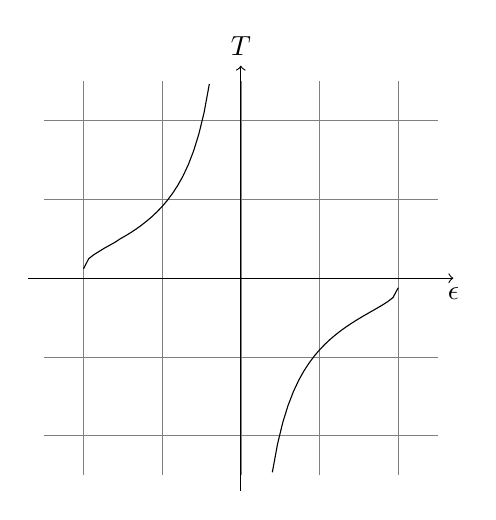
\begin{tikzpicture} [domain=0.4:1.999]
				\draw[very thin, color=gray] (-2.5,-2.5) grid (2.5,2.5);
				\draw[->] (-2.7,0) -- (2.7,0) node[below] {$\epsilon$};
				\draw[->] (0,-2.7) -- (0,2.7) node[above] {$T$};
				\draw[color=black] plot (\x,{-1/ln((1+\x/2)/(1-\x/2))});
				\draw[color=black] plot (-\x,{-1/ln((1-\x/2)/(1+\x/2))});
			\end{tikzpicture}
			\label{fig:paramagnettemperature}
			\caption{Plot of the Temperature of a quantum paramagnet, \eqref{eq:temperatureparamagneticspin}}
		\end{figure}
\end{document}
